\documentclass[border=4pt]{standalone}
\usepackage[utf8]{inputenc}
\usepackage[T1]{fontenc}
\usepackage{lmodern}
\usepackage{amsmath,amssymb,mathtools}
\usepackage{tikz}
\usetikzlibrary{calc,decorations.pathreplacing,angles,quotes}
\usepackage{pgfplots}
\pgfplotsset{compat=1.18}
% Figura extraída de la Tarea 11 de Cálculo I (primer semestre).
\begin{document}
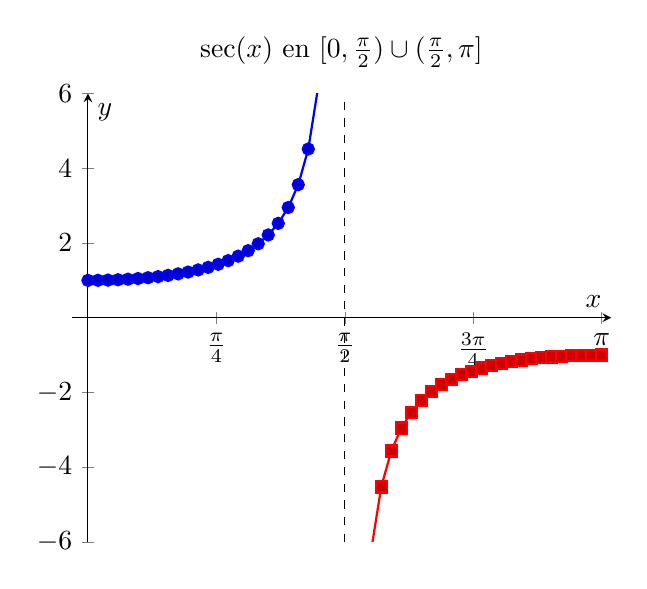
\begin{tikzpicture}
        \begin{axis}[
        xmin=-0.1,xmax=3.2,ymin=-6,ymax=6,
        axis lines=middle,xlabel={$x$},ylabel={$y$},
        xtick={0,0.7854,1.5708,2.3562,3.1416},
        xticklabels={0,\(\tfrac{\pi}{4}\),\(\tfrac{\pi}{2}\),\(\tfrac{3\pi}{4}\),\(\pi\)},
        title={\(\sec(x)\) en \([0,\tfrac{\pi}{2})\cup(\tfrac{\pi}{2},\pi]\)}
        ]
        \addplot+[thick,domain=0:1.47]{1/cos(deg(x))};
        \addplot+[thick,domain=1.671:3.1416]{1/cos(deg(x))};
        \draw[dashed](axis cs:1.5708,-6)--(axis cs:1.5708,6);
        \end{axis}
    \end{tikzpicture}
\end{document}
